Our evaluation quantitatively demonstrates that \sys (i) \emph{reduces memory
protection overhead}, (ii) \emph{improves execution speed} in most cases,
and (iii) \emph{is able to progress} where static systems suffer from a task non-termination loop. 
%
\subsection{Characterization of Overhead}
\label{sec:coala_overhead}

To characterize Coala's overhead we experimented with WISP positioned at
15\,cm away from the signal generator antenna.
We have broken down \sys's overhead to explain the source of its improved performance.

\paragraph{Overhead Reduced by Coalescing.}
\label{sec:overhead-coalescing}

\begin{figure}
    \centering
    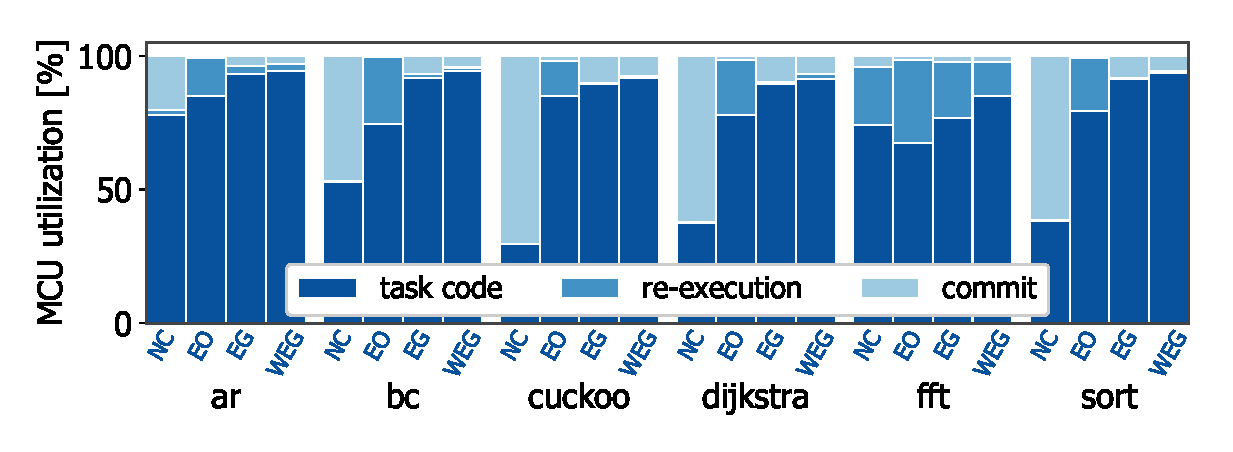
\includegraphics[width=.8\columnwidth]{figures/coalEfficiency}
    \caption{Breakdown of overhead for the proposed coalescing strategies:
    NC (no coalescing), EO (energy-oblivious), EG (energy-guided), WEG
    (weighted energy-guided). All coalescing strategies reduce total
    overhead and maximize useful work. EG and WEG perform better than EO.}
    \label{fig:overallOverheadBreakdown}
\end{figure}

For each coalescing strategy from Section~\ref{sec:task_adaptation} (EO, EG,
and WEG) and for a baseline without coalescing (NC), we have measured the time
spent on executing (i) useful task code, (ii) task code wasted due to a power failure, and
(iii) commits to non-volatile memory at the end of each (coalesced)
task.
%
The overhead incurred by each coalescing strategy is broken down in
Fig.~\ref{fig:overallOverheadBreakdown}. Without coalescing enabled (NC), the
re-execution penalty is the smallest, because the amount of work that can happen
between commits and may have to be re-executed if interrupted is reduced when
work from multiple static tasks is not combined.
%
However, any gain from a reduced re-execution penalty is canceled out by
the increased commit overhead that is incurred at the end of each static
task.
%
Across all benchmarks, all coalescing strategies reduce more commit overhead
than the re-execution overhead they add.
%
This net overhead reduction is greatest in EG and WEG strategies compared
to the EO strategy. We attribute this discrepancy to EO's slow adjustment
of the coalescing target without regard to the energy conditions.
%
In the subsequent experiments, we focus on the better-performing EG and WEG.

\paragraph{\sys's Kernel Overhead.}
%
Fig.~\ref{fig:kernel-overhead} breaks down the time spent on executing 
user task code versus the time spent on kernel operations.
When coalescing is not enabled the commit overhead is highest.
%
The overhead for memory accesses increases in percentage when enabling coalescing,
but not in absolute terms.
%
For both coalescing strategies (EG and WEG) accesses to protected variables
constitute about 30\% of the runtime overhead. Dynamic address translation
necessary on each protected access is the most critical bottleneck for \sys.

\begin{figure}
    \begin{subfigure}{\columnwidth}
			\centering
        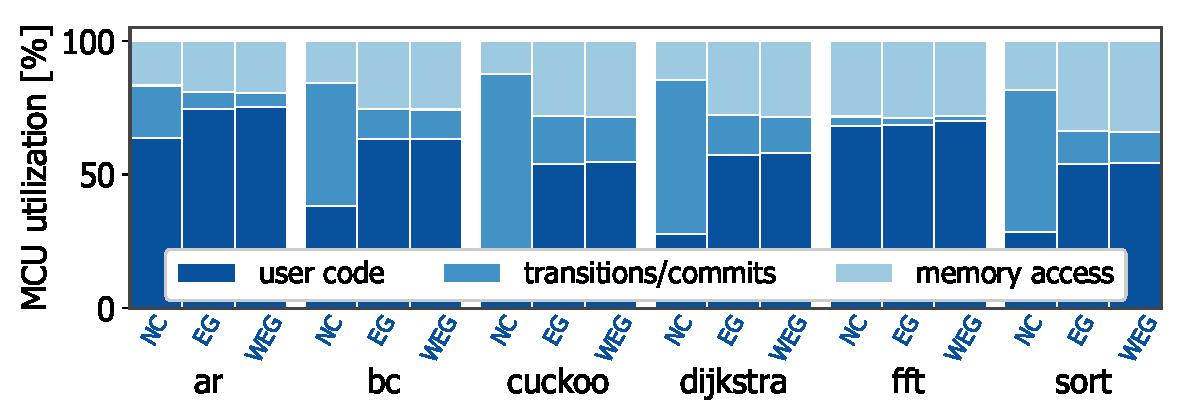
\includegraphics[width=.8\columnwidth]{figures/overallOverhead.pdf}
        \caption{Kernel overhead breakdown}
        \label{fig:kernel-overhead}
    \end{subfigure}
    \begin{subfigure}{\columnwidth}
			\centering
        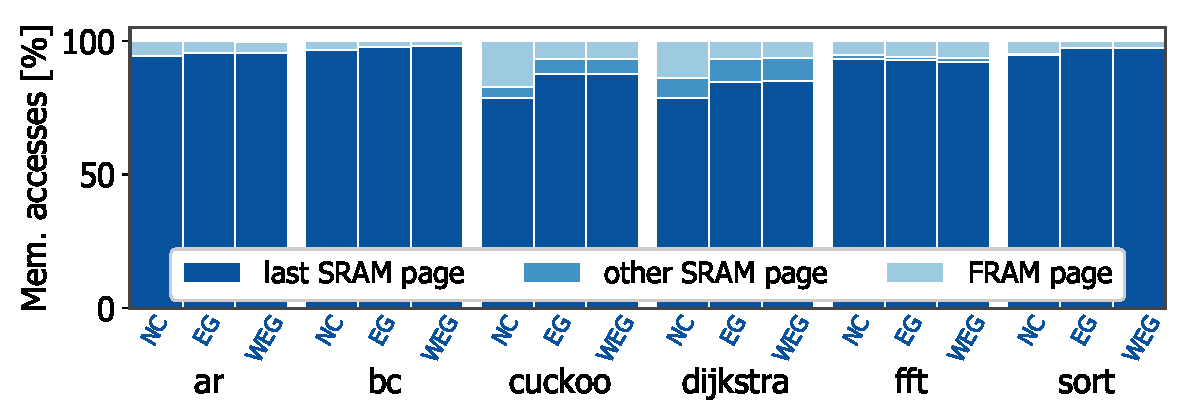
\includegraphics[width=.8\columnwidth]{figures/memAccess}
        \caption{Protected memory accesses breakdown}
        \label{fig:mem-accesses}
    \end{subfigure}
    \caption{\sys's internal overhead. NC: no coalescing, EG:
    energy-guided, WEG: weighted energy-guided.}
    \label{fig:war}
\end{figure}

\paragraph{Protected Memory Accesses Breakdown.}
%
Fig.~\ref{fig:mem-accesses} breaks down protected memory accesses
into three categories.
%
Each type of protected access incurs a different overhead.
Accessing the most recently used SRAM page is of the cheapest kind.
Accessing a different page in SRAM has a slightly higher cost.
Finally, accessing a page that needs to be swapped in
from FRAM into SRAM is the most expensive.
%
The results in the figure show that the overwhelming majority of accesses are
of the cheapest kind, which motivated us to optimize this accesses in our
implementation.
%
Only \textit{cuckoo}, \textit{dijkstra}, and \textit{fft} have non-negligible
number of accesses to a different SRAM page, which is due to the larger working
set and a less regular access pattern in these applications.
%
In general, memory access patterns are shaped by the application, and the more
program state is protected, the higher the rate of page swaps.
%
\subsection{Execution Time}
\label{sec:result_coalescing}
%
Having shown in Section~\ref{sec:coala_overhead} that coalescing reduces
overhead, we now investigate the outcome of this reduction on the total
execution time. We first investigate different variants of \sys and
then compare the best variant to Alpaca~\cite{alpaca}. Additionally, we compare \sys
performance running with different energy buffer sizes. 

\paragraph{Speedup with Coalescing.}
%
\begin{figure}
    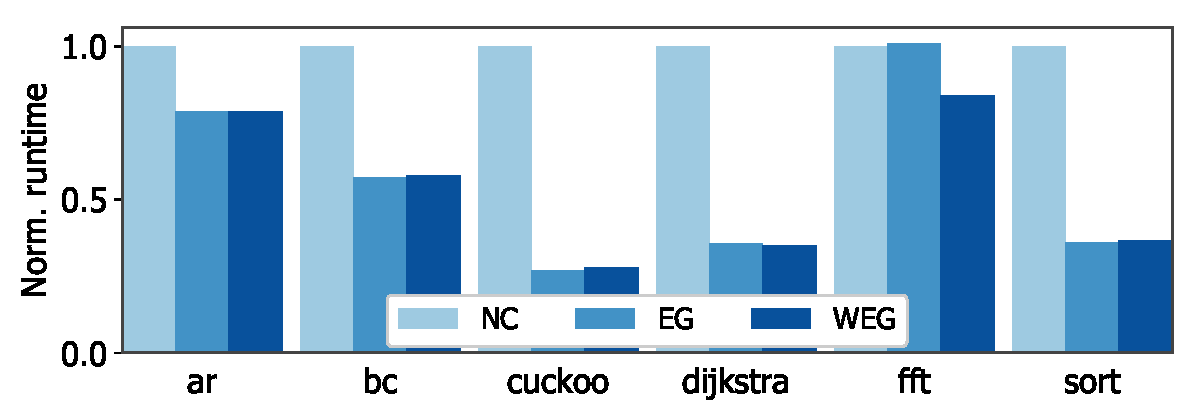
\includegraphics[width=.8\columnwidth]{figures/coalStrategies}%
    \caption{\sys's coalescing performance. Application execution time
with coalescing (EG and WEG) normalized to the execution time
without coalescing (NC).}
\label{fig:coalescing}
\end{figure}

\begin{table}[t]%

\caption{Comparison of \sys performance running the \textit{sort} application on two different capacitor sizes. We see that \sys optimizes its coalesced task size based on the energy buffer size.
\textbf{Coalesced task} refers to the first coalesced task after a reboot, \textbf{Exp. time} shows the experiment duration, the \textbf{Runs} column lists the number of complete runs of the application during the experiments. \textbf{Run time} is the device collective uptime needed to finish a single iteration of the \textit{sort} application.}
\label{tab:dif_cap}

\begin{minipage}{\columnwidth}
\begin{center}
\begin{tabular}{llllll}
  \toprule
    \textbf{Cap. size} ($\mu\text{f}$)& \textbf{Exp. time} ($s$)& \textbf{Duty cycle} & \textbf{Coalesced task} ($ms$)   & \textbf{Runs} & \textbf{Run time} ($ms$) \\
        \hline
    47                 &1205             & 12.93\%    & 33                        & 85       & 183      \\
    470                &1205             & 12.79\%    & 88                        & 87       & 177 \\
  \bottomrule
\end{tabular}
\end{center}
\end{minipage}  
\end{table}%

Fig.~\ref{fig:coalescing} shows \sys's run time of two coalescing
strategies (EG, WEG) normalized to the run time without coalescing (NC).
%
The results show that all benchmarks
complete faster with coalescing than without coalescing: from 25\%
(\textit{ar}) up to 70\% (\textit{sort}).
%
This speedup is a consequence of the reduced overhead demonstrated in
Section~\ref{sec:coala_overhead}.
%
However, the magnitude of the speedup is (1) highly application-dependent and
(2) largely similar across the two coalescing strategies, with the exception of
\textit{fft}.
%
In some cases (\textit{bc}, \textit{cuckoo}, \textit{sort}) WEG's task weighting
system is counter-productive.
%
This occurs in task decompositions with energy-uniform tasks, where counting
tasks disregarding their energy consumption provides an equal amount of information
with a smaller effort.
%
In \textit{fft}, tasks are not uniform, and accounting for their different weights is
beneficial. In fact, the lack of task energy awareness is detrimental: with EG
\textit{fft} runs slower than without any coalescing (NC).
%
The speedup is highest for \textit{bc}, \textit{cuckoo}, \textit{dijkstra} and
\textit{sort}, because their tasks are relatively small and are easily coalesced.
%

\begin{figure}
    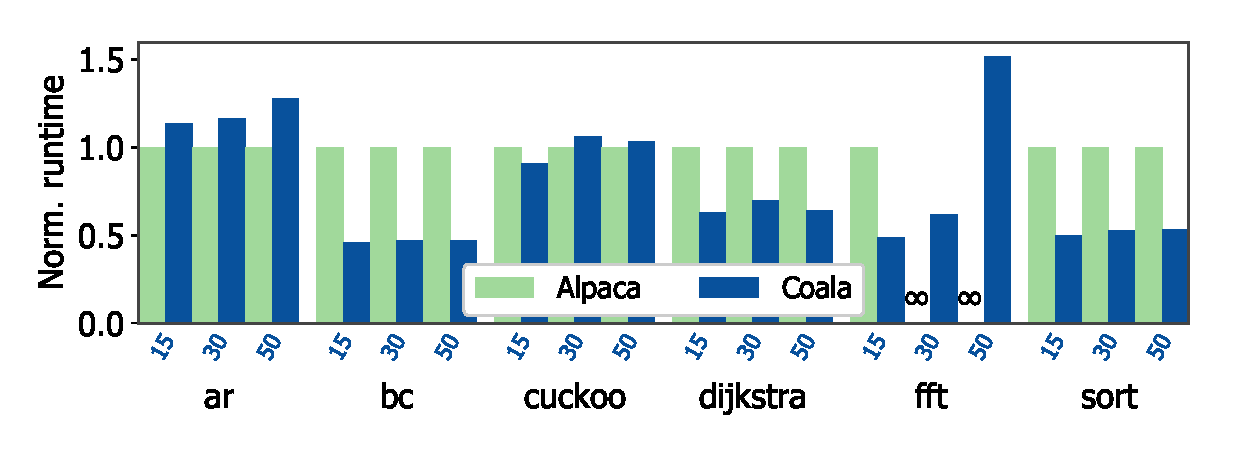
\includegraphics[width=.8\columnwidth]{figures/coala_alpaca_gcc}
    \caption{\sys's execution time normalized to Alpaca's,
    for three distances from the energy source (15, 30 and 50\,cm). }
    \label{fig:runtime}
\end{figure}

\paragraph{Benefits of Adaptive Tasks.}
%
We now compare \sys's performance to Alpaca~\cite{alpaca}---a
\emph{non-adaptive} task-based system with tasks fixed at compile-time.
Fig.~\ref{fig:runtime} shows the average execution time of each
application for \sys and Alpaca, normalized to the latter or, when not possible, to one second.
\sys provides a performance benefit compared to Alpaca for most
applications. For example, it is 54\% faster than Alpaca when executing the \textit{bc} application. In general, the speedup is greatest for applications with repeated WAR
dependencies throughout their code, particularly involving arrays
(\textit{dijkstra}, \textit{fft} and \textit{sort}). \sys's VMM
successfully amortizes the overhead of protecting memory that is accessed in
such patterns.  In applications without locality among accesses to protected
variables \sys incurs overhead from memory
virtualization that causes its performance to be comparable to (or worse than)
Alpaca (\textit{ar}, \textit{cuckoo}).

Due to its static progressing behavior, Alpaca was unable to complete the \textit{fft} benchmark on distances larger than 15\,cm\footnote{At distances greater than 15\,cm, energy incoming during
execution is negligible and the stored energy is insufficient to complete some of
the static tasks.}. This is marked with $\infty$ signs in Fig.~\ref{fig:runtime}. \sys, however, managed to complete \textit{fft} by enabling its task downscaling at 30\,cm and 50\,cm from the energy source.

\paragraph{Different Capacitor Sizes}
Table~\ref{tab:dif_cap} shows how \sys optimizes its Coalescing task size based on the amount of buffered energy.
We see that \sys scales up its coalesced task size with a bigger energy buffer and vice versa. This allows it to reduce the time-to-completion of the applications. For example, 
the \textit{sort} run-time is reduced from 183\,ms to 177\,ms when the capacitor is changed from 47\,$\mu$F to 470\,$\mu$F. It should be emphasized that a device with a bigger energy buffer suffers less from power failures (but requires longer charging time). However, as has been measured in Fig.~\ref{fig:overallOverheadBreakdown} and explained in Fig.~\ref{fig:coal_anatomy}, the re-execution penalty for the \textit{sort} application is negligible.  

 
Overall, \sys shows better performance than its counterpart, and it is able to overcome the \textit{big task} (i.e. \textit{fft} tasks) problem that the static task-based systems suffer from. 

\subsection{Virtual Memory Performance}
\label{sec:results_memory_management}

We characterize the performance of \sys's virtual memory sub-system in an
experiment on a continuously-powered evaluation board, as described in
Section~\ref{sec:results_hardware_software}.
% Fig.~\ref{fig:page_size} quantifies the effects of page size.

\begin{figure}
	\centering
    \begin{subfigure}{\columnwidth}
			\centering
        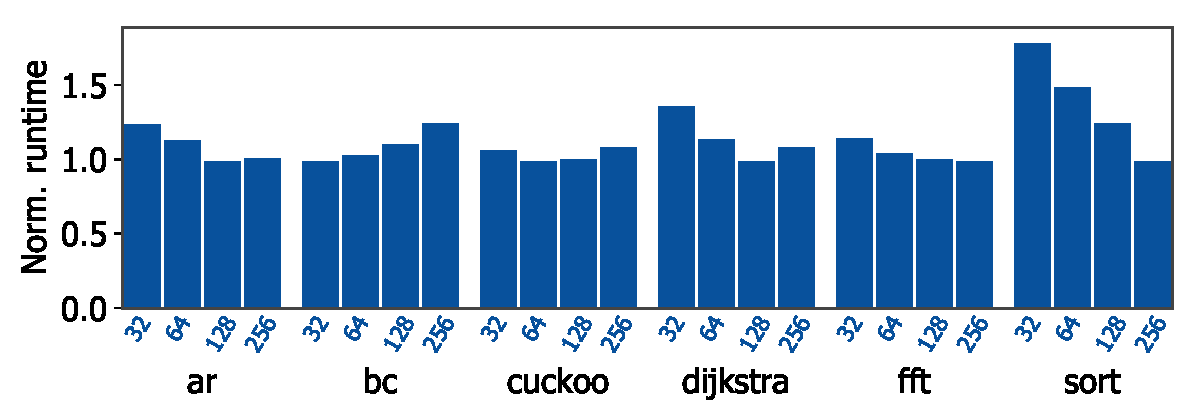
\includegraphics[width=.8\columnwidth]{figures/page_exec-time.pdf}
        \caption{Execution time normalized to lowest per-application}
        \label{fig:page-exec-time}
    \end{subfigure}
    \begin{subfigure}{\columnwidth}
			\centering
        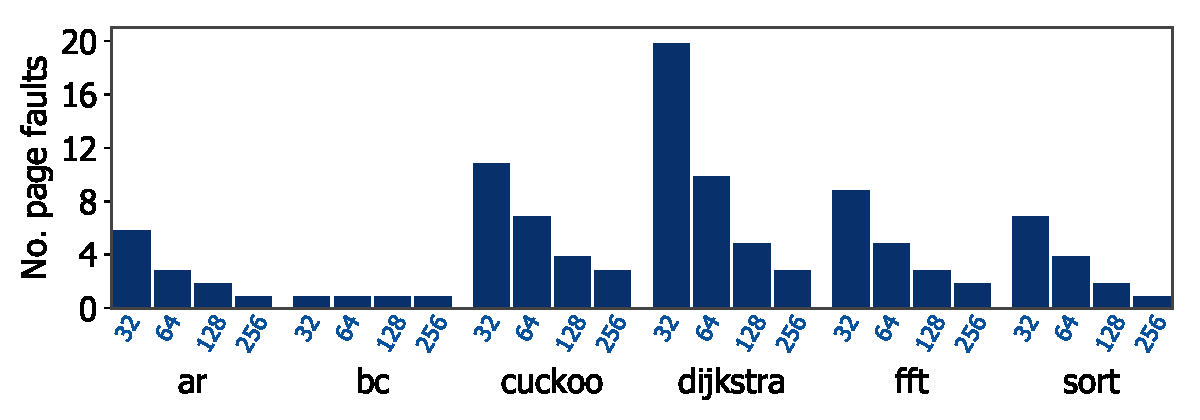
\includegraphics[width=.8\columnwidth]{figures/pagePulls.pdf}
        \caption{Number of page faults per application run}
        \label{fig:page-pulls}
    \end{subfigure}
    \caption{Effect of page size (in bytes).}
    \label{fig:war}
\end{figure}

\paragraph{Effect of Page Size on Runtime.}

Fig.~\ref{fig:page-exec-time} shows the execution time as a function
of page size (in bytes), normalized to the lowest per-application performance among the
set of page sizes.
The data suggest that there is a page size that minimizes execution time.
The best page size is not the same for
each application. Nevertheless, if a choice must be made for all applications,
128-B pages are the best option.

\paragraph{Effect of Page Size on Page Faults.}

Fig.~\ref{fig:page-pulls} reports the number of page faults, per application
run, as a function of page size (in bytes).
%
The smaller the page the more likely that a memory access will land
outside that page and that a new page will have to be swapped in.
%
This trend is visible for all applications, except for \textit{bc}. The total
amount of data accessed by \textit{bc}, as well as its working set, is small.
Even with the smallest page, all accesses are contained within that page, and
no page fault occurs. Without any page faults to begin with, increasing the
page size only yields overhead.
